\documentclass[10pt]{article}
\usepackage[margin=0.82in]{geometry}
\usepackage[T1]{fontenc}
\usepackage{lmodern,microtype,booktabs,array,tabularx,graphicx,xcolor,tikz,amsmath}
\usetikzlibrary{arrows.meta,positioning,fit}
\usepackage[numbers,sort&compress]{natbib}
\usepackage{enumitem,url,hyperref}
\definecolor{palblue}{HTML}{245A7A}
\definecolor{palgreen}{HTML}{2D7B64}
\definecolor{palgold}{HTML}{B27A20}
\definecolor{palred}{HTML}{9E3D38}
\hypersetup{colorlinks=true,linkcolor=palblue,citecolor=palgreen,urlcolor=palblue}
\setlist{nosep,leftmargin=*}
\setlength{\parskip}{0.25em}
\setlength{\parindent}{0pt}
\newcommand{\pending}{\textbf{PENDING}}
% Never fall back to historical claims.tex or development smoke measurements.
\InputIfFileExists{generated/authority-claims.tex}{}{}
\providecommand{\StudyCommit}{\pending}
\providecommand{\ProtocolHash}{\pending}
\providecommand{\StudyDeclaredUnits}{111}
\providecommand{\StudyCompletedUnits}{\pending}
\providecommand{\FaultDeclaredUnits}{50}
\providecommand{\FaultCompletedUnits}{\pending}
\providecommand{\FaultBaselineFalseAccepts}{\pending}
\providecommand{\FaultBaselineKnownClaims}{\pending}
\providecommand{\FaultBaselineUnknownClaims}{\pending}
\providecommand{\FaultSystemSilentAccepts}{\pending}
\providecommand{\FaultBenignFalseRejects}{\pending}
\providecommand{\ContinuationPassed}{\pending}
\providecommand{\ContinuationDeclared}{10}
\providecommand{\ReplayPassed}{\pending}
\providecommand{\ReplayDeclared}{5}
\providecommand{\OverheadMatchedSeeds}{\pending}
\providecommand{\OverheadDeclaredSeeds}{10}
\providecommand{\SynchronousOverheadMedian}{\pending}
\providecommand{\BackgroundOverheadMedian}{\pending}
\providecommand{\StorageOverheadMedian}{\pending}
\providecommand{\NullWallMedianMs}{\pending}
\providecommand{\StorageWallMedianMs}{\pending}
\providecommand{\OfflineStatus}{\pending}
\newcommand{\studyinput}[1]{\InputIfFileExists{generated/#1.tex}{}{\par\fbox{\parbox{0.92\linewidth}{\pending: frozen campaign output #1 has not been bound to this draft.}}\par}}
\title{Who Changed the World?\\Authority-Aware Replay for Interactive Embodied-AI Experiments}
\author{Anonymous authors\\\small Venue-neutral research draft}
\date{November 2026}
\begin{document}
\maketitle
\begin{abstract}
An interactive controller experiment can accept an intervention before applying
it, restore a pose without restoring recurrent state, or replay a trajectory
without executing its policy. Each operation can finish successfully while
supporting a weaker claim than its reader assumes. We present Palimpsest, an
experiment layer that composes applied-command receipts, controller-visible
observations, complete continuation state, declared replay computations, and
retained evidence. Its contract makes the operation performed and the fields
validated independently inspectable. We test the thesis that these semantics
expose evidence errors admitted by explicitly weak acceptance predicates while
preserving executable continuation and replay at measured cost. The frozen
CPU study contains 50 fault/challenge units, 10 continuation pairs, five replay
trajectories, 10 four-condition overhead sets, five operation-cost units, and
one same-host fresh-checkout check. Campaign results are \pending{} in this draft;
no outcome is inferred from the expected fault response. The contribution is a
composed semantic contract and its controlled evaluation, rather than a new
replay taxonomy or a performance ranking of existing systems.
\end{abstract}

\section{Introduction}
Suppose an experimenter adds an obstacle while a recurrent controller navigates
a simulated world. The browser draws the obstacle immediately; the server
accepts the request, but its application waits for a later control boundary.
A saved trajectory subsequently plays without error. Did the controller react
to that obstacle, and did replay reproduce its computation? Request acceptance
and visual similarity cannot answer either question. The obstacle might not
have entered the authoritative world at the displayed tick, and the replay
might simply display saved values. This is a hypothetical interpretation error,
not a measured account of user behavior. Our evaluation injects these conditions
directly and retains their observable consequences.

The stakes are causal as well as operational. An intervention claim ties a
change to a decision boundary. A continuation claim ties future behavior to a
restored state. A policy-reproduction claim ties agreement to a computation that
actually executed. A successful HTTP response, advancing simulator, or parseable
artifact is useful evidence, but it does not establish all three relationships.
An experiment layer should preserve enough structure to test them separately.

Existing systems already distinguish important parts of this problem.
robomimic provides recorded-observation visualization, simulator-state playback,
and open-loop action playback; ManiSkill distinguishes action replay from
state-based playback and documents nondeterminism
\citep{robomimicplayback,maniskillreplay}. MuJoCo documents the state needed for
continuation and its reproducibility scope \citep{mujococomputation}.
We build on those distinctions. The remaining design question is how an
interactive lab can connect applied authority, controller-visible input,
recurrent continuation, replay execution, and evidence admission into one
checkable account.

Our thesis is falsifiable: \emph{explicit authority and replay semantics expose
silent evidence errors admitted by specified weak acceptance predicates,
while preserving declared continuation and replay at measured cost.}
A contract violation that the system silently admits challenges the first part;
a full-state continuation or declared replay that disagrees challenges the
second. Cost is measured without an ``acceptable overhead'' threshold. Weak
predicates are intentionally named assumptions evaluated on the same traces,
not implementations attributed to another software project.

Palimpsest wraps a pinned MuJoCo/FLYNN execution path. One runtime owner commits
interventions at control boundaries and emits receipts describing what happened.
Snapshots include recurrent and application state as well as physics. Replay
outputs declare both executed computation and validated fields. Bounded writers
retain a valid prefix without elevating partial publication to terminal success.
The instrument is the subject; navigation quality is not the outcome.

The paper makes three contributions:
\begin{enumerate}
\item A semantic contract joining applied intervention authority, continuation
state, replay execution, and terminal evidence, with explicit failure boundaries.
\item An implementation of that contract using boundary receipts, observation
projection, complete snapshots, independent branch owners, and bounded staged
publication.
\item A frozen, paired evaluation separating fault detection, executable
agreement, execution overhead, operation cost, and same-host reproducibility.
\end{enumerate}

\section{Failure Model and Semantic Contract}
\label{sec:contract}
\subsection{What must a trace distinguish?}
Let $x_t$ be authoritative simulator and application state immediately before
control tick $t$, $h_t$ controller state, and $r_t$ the state of random generators.
A projection $P$ produces the permitted observation $o_t=P(x_t)$; the controller
computes $(a_t,h_{t+1})=\pi(o_t,h_t)$, and physics advances under $a_t$.
The browser can display a separate state $d$ at a different cadence. Neither
$d$ nor a command request is an input to this transition until the owner commits
an appropriate change.

A submitted command $c$ has an identity, expected revision, and payload.
An acceptance acknowledges queue admission. An applied receipt names its
actual control tick and resulting revision. A rejection or failure has a
different terminal meaning. Delayed execution is permitted; silently treating
admission as application is not. Duplicate command identities must not produce
duplicate application. A stopped or interrupted run may leave an unresolved
accepted command; a retained prefix must preserve that uncertainty rather than
invent a terminal receipt.

A continuation state is sufficient only relative to the next transition.
Matching $qpos$ and $qvel$ can leave recurrent hidden state, retinal processing,
wrapper counters, randomized inputs, or pending commands different. A branch
additionally requires independence: mutating a child must not mutate its parent
or sibling. Sequential scheduling alone does not guarantee independence if
mutable owners are shared.

Replay has two orthogonal dimensions: what executes and what is compared.
Playback reads recorded values. Action replay advances physics using recorded
actions while bypassing policy inference. Policy replay recomputes controller
outputs as the reconstructed experiment advances. Agreement of an output
trajectory cannot establish an unexecuted policy computation. Conversely,
executing inference without comparing its scientific outputs does not establish
agreement. Figure~\ref{fig:matrix} makes this separation operational.

\subsection{Three obligations}
\textbf{I1: application has an authority boundary.}
Only one owner mutates the live simulator/controller state. An application
has one authoritative receipt and control tick. Expected revisions are checked
at application, and duplicate identities cannot apply twice. Normal command
completion resolves admission into an applied, rejected, or failed outcome;
interruption does not acquire a success meaning by default.

\textbf{I2: continuation binds transition-relevant state and identity.}
Restore requires a compatible schema, source and asset identity, physics state,
controller state, wrapper state, random state, and pending application state.
Missing or incompatible required components must be refused before mutating the
destination. Branches instantiate separate mutable owners and preserve their
source object. Equal initial pose is an insufficient acceptance condition.

\textbf{I3: evidence names its computation and publication status.}
Every replay declares its mode, whether inference executed, its comparison
fields and tolerances, and agreement or first divergence. Outputs use a new
destination. Readers distinguish a validated published prefix from terminal
completion; the presence of an output directory never establishes the latter.
These obligations concern supported statements about a run, rather than a
promise that every run completes or agrees.

\subsection{Threat boundary}
The fault model includes asynchronous admission and delayed application, stale
revisions, duplicate requests, omitted state, source/asset drift, shared mutable
branches, interrupted publication, quota exhaustion, queue saturation, and
writer failures. We exercise runtime faults through the CPU controller path and
storage faults through production interfaces with controlled payloads.
We trust the host OS, runtime owner, instrumentation, and measurement code.
File identity and protected rechecks detect specified custody changes; they do
not defend against a hostile kernel or prove every transient mutation was
observed. Staged publication is an application protocol, not power-loss crash
consistency. These boundaries determine what the following mechanisms can claim.

\section{Design and Implementation}
\subsection{Receipts at control boundaries}
The browser and CLI submit commands to a bounded queue rather than mutating
physics directly. The owner holds the simulator, controller, renderer, recorder,
and command state. A preview can check shape and geometry, but the owner
revalidates the command at the boundary where it would take effect. It then
applies the mutation, refreshes dependent state, and records the application
revision and tick. A stale preview cannot authorize a later mutation against a
new revision. Receipts make delay and refusal visible without requiring the
interface frame cadence to match the controller cadence.

\begin{figure}[t]
\centering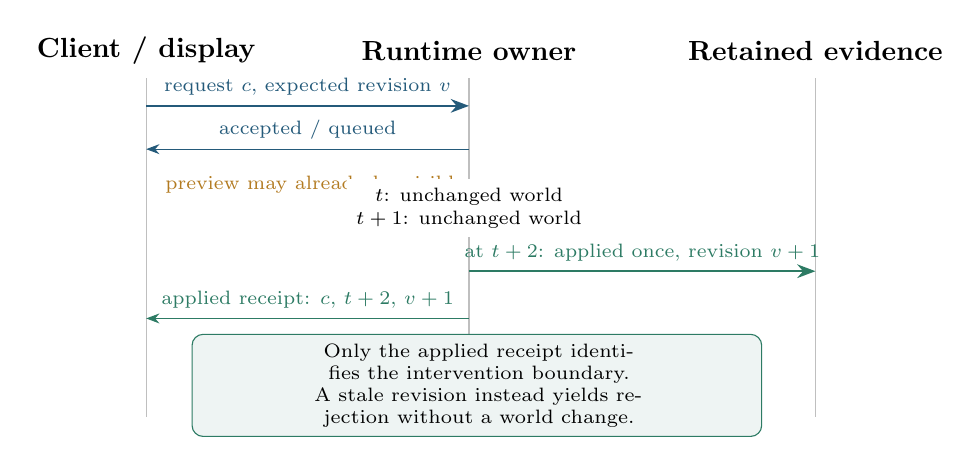
\begin{tikzpicture}[x=1cm,y=1cm,>=Stealth,font=\small]
\node[font=\bfseries] at (0,0) {Client / display};
\node[font=\bfseries] at (4.1,0) {Runtime owner};
\node[font=\bfseries] at (8.5,0) {Retained evidence};
\foreach \x in {0,4.1,8.5} \draw[gray!50] (\x,-0.35)--(\x,-4.65);
\draw[->,thick,palblue] (0,-0.7)--node[above,font=\scriptsize]{request $c$, expected revision $v$}(4.1,-0.7);
\draw[->,palblue] (4.1,-1.25)--node[above,font=\scriptsize]{accepted / queued}(0,-1.25);
\node[anchor=west,font=\scriptsize,text=palgold] at (0.12,-1.7) {preview may already be visible};
\node[fill=white,font=\scriptsize,align=center] at (4.1,-2.0) {$t$: unchanged world\\$t+1$: unchanged world};
\draw[->,thick,palgreen] (4.1,-2.8)--node[above,font=\scriptsize]{at $t+2$: applied once, revision $v+1$}(8.5,-2.8);
\draw[->,palgreen] (4.1,-3.4)--node[above,font=\scriptsize]{applied receipt: $c$, $t+2$, $v+1$}(0,-3.4);
\node[fill=palgreen!8,draw=palgreen,rounded corners,align=center,font=\scriptsize,text width=7cm] at (4.2,-4.25) {Only the applied receipt identifies the intervention boundary.\\A stale revision instead yields rejection without a world change.};
\end{tikzpicture}

\caption{An accepted intervention waits while the authoritative world remains
unchanged. Only the owner's receipt at symbolic tick $t+2$ supports an applied
claim. The diagram illustrates the contract; it is not a measured latency trace.}
\label{fig:authority}
\end{figure}

Idempotent command identities protect against retry duplication; the receipt
records one application rather than equating each acknowledged request with a
new intervention. Dropping presentation frames is compatible with this contract,
but dropping authoritative events is not. This choice trades UI simplicity and
maximum throughput for an explicit serialization point. The serialized boundary
also makes snapshots and later replay interpretable: a snapshot belongs before
or after a recorded application, rather than somewhere inside an unrecorded
concurrent mutation.

\subsection{Observation projection records the information boundary}
A simulator typically exposes more information than a policy should consume.
Palimpsest projects declared policy inputs from the authoritative world and
keeps projected observations separate from world truth and display metadata.
This distinction matters even when values happen to coincide. A goal location
available to an inspector is not automatically evidence that the learned policy
received it; a displayed obstacle is not automatically evidence that the policy's
camera saw it.

Typed records retain policy inputs and outputs alongside physical fields.
Comparisons can therefore locate whether disagreement begins in observation,
controller response, or dynamics. Projection makes the information boundary
inspectable, but it is not an information-flow proof of all upstream code.
Additional controller profiles require an explicit projection and state adapter;
the runtime cannot infer an unknown policy's hidden dependencies.

\subsection{Snapshots capture a continuation, not a picture}
Snapshots combine native physics state and mutable world properties with
controller hidden/retinal state, wrapper counters, random-generator state,
recorder position, and pending commands. Source and asset fingerprints bind the
snapshot to the implementation and graph/checkpoint/mapping identities that
interpret it. Shape compatibility alone is inadequate: a different checkpoint
can load while changing the transition function.

MuJoCo's own state and reproducibility documentation motivates preserving
integration and warm-start state \citep{mujococomputation}. Palimpsest adds the
application and recurrent-controller components around that physics boundary.
Restore validates the payload and identities before destination mutation.
A source snapshot remains a retained object; a branch restores into a separate
owner and produces a new run. Branches execute sequentially in this study to
avoid shared simulator state and resource contention, at the cost of parallel
exploration throughput.

Full snapshots are larger and more version-sensitive than pose files. That
cost buys a testable continuation claim: the source and restored execution can
be compared over future ticks, including controller state. It does not buy
universal determinism across versions or architectures. A newly supported
component must identify all state that can affect the next transition or refuse
the stronger resumability claim.

\subsection{Replay declares execution and comparison}
\begin{figure}[t]
\centering\renewcommand{\arraystretch}{1.3}
\begin{tabularx}{\linewidth}{@{}l c c X@{}}
\toprule
Operation & Run physics & Run policy & Representative records and validation\\
\midrule
Playback & No & No & Display recorded cameras, poses, actions and available controller records; no physics or policy recomputation.\\
Action replay & Yes & No & Compare cameras/sensors, actions/control, pose/next pose, reward, simulation time and revision. Controller records are not recomputed.\\
Policy replay & Yes & Yes & Recompute and compare physical fields and controller encoded input/raw output; report first divergent field/tick under declared tolerances.\\
\bottomrule
\end{tabularx}

\caption{Replay modes differ in computation as well as validation. A physical
match under recorded actions leaves policy recomputation untested. The matrix
specifies Palimpsest's modes; it does not classify competing systems.}
\label{fig:matrix}
\end{figure}
The executable replay path checks source, asset and snapshot compatibility,
creates a new destination, restores initial state, and advances the declared
computation. Action replay restores a compatible controller for state loading
but bypasses inference. Policy replay executes it and compares the richer
record. Reports retain mode, inference execution, agreement, and first divergent
field/tick. New run IDs and measurement latencies are not scientific equality
requirements; identity provenance still remains inspectable.

The study's R1/R2 challenges deliberately relabel playback or action replay as
policy reproduction and apply an execution-label guard. That guard is a
\emph{study-level claim-admission check}. It must not be read as evidence that
the production playback interface was independently asked for, and refused,
a mislabeled policy operation. Production compatibility refusals in source,
asset, or snapshot cases exercise a different mechanism. Keeping those paths
separate prevents a successful test oracle from being reported as a production
feature it did not exercise.

\subsection{A valid prefix is not terminal publication}
The recorder writes typed numeric chunks and ordered events under bounded byte,
count, queue, and free-space policies. Staging and no-overwrite publication
separate prepared bytes from admitted objects. A reader follows the published
record rather than treating every file left in the directory as valid data.
An interruption can therefore leave a useful validated prefix and an ignored
unpublished tail, without a terminal-success claim.

A background writer decouples some producer work from storage latency, but a
bounded queue must apply backpressure rather than silently discard accepted
items. Writer errors become terminal failures and release resources; an
attempted write is not a completed artifact. Synchronous writing gives a simpler
completion boundary while putting more work on the control path. The overhead
experiment measures this tradeoff directly.

Protected readers also recheck file identities around guarded reads. At and
below a declared custody root, namespace and content participate in the check;
above that root, parent-edge identity is retained without interpreting unrelated
sibling churn as a mutation of protected evidence. This avoids making benign
activity elsewhere on the host a reason to reject an unchanged source. Checks
are bounded to the declared custody operation rather than advertised as global
filesystem surveillance.

\section{Evaluation}
\label{sec:evaluation}
\subsection{Protocol and interpretation}
The predeclared protocol was committed and then frozen; it is not an independent
public preregistration. Seed 0 appeared in disclosed harness-development smoke
checks, so the fixed seeds support engineering repeatability, not held-out
evaluation. The study asks four questions: (RQ1) which injected evidence errors the
contract exposes; (RQ2) whether complete continuation and declared replay agree;
(RQ3) what execution and operation costs the mechanisms incur; and (RQ4) whether
a fresh checkout on the same host can execute the focused workflow.
The controller is pinned CPU FLYNN, a recurrent navigation model constrained by
fly-brain topology \citep{wang2026flynn}, executed in MuJoCo. There is no model
training, controller tuning, held-out evaluation, or competing-system benchmark.

The protocol declares 111 invocation descriptors: 50 fault/challenge units,
10 continuation pairs, five replay trajectories, 40 execution-overhead
invocations forming 10 four-condition matched sets, five operation units, and
one offline check. A seed identifies an engineering repetition, not a sampled
independent environment. A continuation pair and a replay trajectory are their
respective units; ticks within them are repeated measurements. Fault units are
specified case/condition/repetition executions, including deterministic fixture
variants. Failures, refusals, timeouts, and incomplete units remain in declared
denominators and cannot be replaced with successful retries.

The campaign runs sequentially under a four-hour limit, 900 seconds per unit,
a 16 GiB logical-output cap, and a 6 GiB actual free-space reserve. Ordinary
units permit 512 MiB; the fresh-checkout unit permits 10 GiB logical inventory
because its dependency environment is included. Crossing a resource or timeout
boundary stops new work and retains completed and partial records. These
execution limits control the study; they do not constitute measured overhead
acceptance thresholds.

\paragraph{Frozen comparison policy.}
Scientific arrays must be finite: NaN and infinity are rejected, even at matching
positions. Float32 physics/controller arrays use absolute and relative tolerances
of $10^{-6}$; integer, Boolean, identity, shape, and event fields follow the
frozen exact comparison policy. Source/asset identities must match exactly.
First divergence names a field and tick. The study-level finite/exact checks
supplement production replay reporting; the claim is about their evaluated
composition. Scope is CPU, same version, same architecture.

\paragraph{Result binding.}
The campaign execution commit is \StudyCommit{} and protocol digest is
\ProtocolHash{}. Completed descriptors: \StudyCompletedUnits{}/\StudyDeclaredUnits{}.
\textbf{Result interpretation remains pending until the retained campaign summary
is bound and checked.} Generated tables are the only numerical result source;
prior controller smoke tests and historical capability studies are excluded.

\subsection{RQ1: Semantic errors and explicit acceptance predicates}
The 50 units cover delayed/stale/duplicate intervention requests (A1--A3), replay
mislabeling (R1--R2), incomplete snapshots (S1--S2), source/asset substitutions
(D1--D2), protected custody and benign sibling churn (C1--C3), interrupted
publication (P1), independent/shared-owner branches (B1--B2), and quota, queue,
and writer failures (E1--E3). Runtime cases traverse the actual CPU FLYNN/lab
path; custody, publication and resource cases use production interfaces with
small deterministic fixtures. The table keeps those evidence paths visible.

\begin{table}[t]
\centering\small
\caption{Frozen fault/challenge matrix. Each weak predicate is a stated
acceptance assumption evaluated on the same trace, not a competitor. Acceptance
and observed claim truth must be interpreted separately.}
\label{tab:fault}\studyinput{fault-matrix}
\end{table}

For example, ``accepted request means applied intervention'' admits A1 before
application; ``viewable trajectory means policy reproduced'' ignores whether
inference ran in R1. Pose-only and shared-owner ablations remove specific state
or isolation mechanisms. These intentionally weak checks expose what evidence
is missing from those assumptions. They do not estimate how often scientists
make such mistakes or how another framework would respond.

A predicate's acceptance is also distinct from a false claim. The retained
record names the claim, its temporal scope, and its observed truth as true,
false, or unknown. In particular, B1's separate-owner branch can remain
independent and E2's bounded queue can retain accepted items through backpressure:
these are valid challenges in which acceptance need not be erroneous. Unknown
truth stays unknown rather than being counted as a demonstrated false claim.
C3 provides benign controls for false rejection.

The result counters are \FaultCompletedUnits{}/\FaultDeclaredUnits{} completed
units, \FaultBaselineKnownClaims{} claims with known truth and
\FaultBaselineUnknownClaims{} with unknown truth, \FaultBaselineFalseAccepts{}
measured false acceptances under the weak predicates,
\FaultSystemSilentAccepts{} silent system acceptances, and
\FaultBenignFalseRejects{} benign false rejections. No favorable interpretation
is assigned to these pending counters. A contract refusal counts as detection
only when the named trace and semantic oracle support it; an unrelated crash is
not semantic success.

\subsection{RQ2: Complete continuation and declared replay}
Ten seeds each execute an eight-tick prefix followed by a 100-tick
source/restored continuation comparison. The retained data include paired raw
values, snapshot size and digest, and first divergence. The independent unit is
the seeded pair. Agreement is \ContinuationPassed{}/\ContinuationDeclared{}
under the frozen policy; a passed count is not populated from expected behavior.

Five additional source trajectories each use an eight-tick prefix and 100 source
ticks, followed by branch, playback, action replay, and policy replay conditions.
They share a source, so conditions are paired rather than independent trials.
Playback reports recorded data without executing physics; action and policy
replay must be interpreted through the computation/validation matrix.
The trajectory-level result is \ReplayPassed{}/\ReplayDeclared{}.

\begin{table}[t]
\centering\small
\caption{Continuation and replay outcomes under the frozen comparison policy.
Counts refer to source/restored pairs or source trajectories, never individual
ticks. Executed computation constrains the interpretation of agreement.}
\label{tab:replay}\studyinput{replay-table}
\end{table}

The ablated snapshot and branch challenges test why the full mechanisms are
needed; the complete-state pairs test that enforcing them does not merely refuse
all work. Neither validates biological fidelity or navigation generalization.
Any divergence must remain reported with its original field/tick rather than
being erased by a post-result tolerance change.

\subsection{RQ3: Execution overhead and operation cost}
Ten seeds run four conditions in fresh processes: a benchmark-only null writer,
a synchronous writer, a background writer, and a background writer plus actual
bounded storage accounting. Each uses 20 warm-up ticks and 200 measured ticks.
The null writer isolates recording cost; it is not a reproducibility baseline.
Condition order rotates cyclically by seed modulo four. This balances order
positions across the bounded design without claiming complete randomization.
Caches are warm and the OS page cache is not flushed.

Actions, tick count and final-state match are required across all four
conditions. A mismatched seed retains all four observations and is excluded as
a whole from timing summaries, with its unmatched status reported. Open and
close costs are recorded separately from steady-state wall time per tick.
Instrumentation also records policy/physics/camera time, bytes per tick, peak
RSS, descriptor/thread counts where available, queue backpressure, and storage
recount work. Load, available memory, condition ordinal, readable CPU/governor
identity, and competing Palimpsest processes are retained as covariates.

\paragraph{State matching excludes one identified telemetry field.}
Native MuJoCo state contains elapsed-time telemetry that can differ even when
scientific state agrees. For execution-overhead matching only, the driver zeros
\texttt{timer.duration} on private decoded copies and recomputes the native
hash. Live engine state and retained original snapshots are unchanged. Raw and
matched hashes and the normalization descriptor are retained. Recorder
source-run/event-prefix identities also differ by construction. RNG,
integration, controller, observation, application, solver, physics, and other
serialized cache state remain in the match. This targeted normalization does
not weaken snapshot restoration or replay validation and is not a numerical
result about the campaign.

\begin{table}[t]
\centering\small
\caption{Matched execution cost. All four conditions for a seed enter or leave
the timing summary together. Open and close costs are separate from measured
tick time. No overhead pass threshold is imposed.}
\label{tab:overhead}\studyinput{overhead-table}
\end{table}
\begin{figure}[t]
\centering\studyinput{overhead-plot}
\caption{Paired execution costs by seed and condition. Shared seed identity
supports within-set comparison; plotted samples are not independent ticks.}
\label{fig:overhead}
\end{figure}

The matched-set count is \OverheadMatchedSeeds{}/\OverheadDeclaredSeeds{}.
The generated median overheads relative to null are
\SynchronousOverheadMedian{}\%, \BackgroundOverheadMedian{}\%, and
\StorageOverheadMedian{}\% for synchronous, background, and storage-accounted
conditions respectively. Null and storage-accounted median wall times per tick
are \NullWallMedianMs{} and \StorageWallMedianMs{} ms. These pending quantities
will describe this host and workload; they have no preregistered acceptability
threshold and cannot establish a competing-system performance rank.

Operation costs use the five retained full background-plus-storage source runs
from RQ2. Each unit measures capture, save, read, restore/first-tick, playback,
action replay, and policy replay. Their different computational work is explicit:
playback timing cannot be substituted for policy-replay cost. Null-writer runs
produce no replay timings. Summary statistics and paired values are descriptive;
there is no significance test or operation-cost pass threshold.

\begin{table}[t]
\centering\small
\caption{Operation costs on retained RQ2 source runs. Each seed contributes one
operation unit; capture, serialization, restore, and the replay computations
measure different work.}
\label{tab:operation}\studyinput{operation-table}
\end{table}

\subsection{RQ4: Fresh local checkout}
One offline verifier invocation checks a clean checkout at the frozen source
commit using full FLYNN assets and a bounded 55-second workflow, with setup
included in the unit's resource accounting. Its status is \OfflineStatus{}.
The check tests local packaging and workflow execution with a new checkout;
it retains the same host and asset availability. It cannot answer whether an
independent operator on a second machine can reproduce the experiment.

\section{Related Work}
\paragraph{State playback and action replay already exist.}
The closest semantic precedents are robomimic and ManiSkill.
robomimic's playback script visualizes saved observations, restores simulator
states, or loads an initial state and applies recorded actions open loop
\citep{robomimicplayback}. ManiSkill defaults to action replay and supports
state-based playback, documenting nondeterminism and CPU/GPU replay differences
\citep{maniskillreplay}. These sources already establish that state and action
replay are different operations. Our design adds no priority claim for that
taxonomy. Its focus is a composed contract connecting live applied-command
receipts to recurrent continuation, policy recomputation, and admission of
retained claims. The evaluation compares named predicates and narrow ablations;
it does not benchmark these projects or infer missing features from their docs.

\paragraph{Recording at middleware and simulation layers.}
rosbag2 records and republishes middleware messages \citep{rosbag2}.
CARLA's recorder reenacts actors from recorded states and events
\citep{carlarecorder}. Gazebo logs server information and entity poses,
insertion and deletion; it also supports resource recording and a default that
avoids overwriting an existing log path \citep{gazebologging}.
Those are useful guarantees at their respective layers. Republished messages
or reenacted entities can serve many inspection tasks without claiming to
recompute a recurrent policy. Palimpsest's mode declaration makes that
computational scope part of the experiment report. Bounded recording,
provenance, and no-overwrite behavior are established techniques, not unique
contributions individually.

\paragraph{Physics continuation and process replay.}
MuJoCo explains integration-state restoration, warm-start requirements, and
same-version/architecture limits \citep{mujococomputation}. Palimpsest relies on
that substrate and captures the surrounding recurrent-controller and application
state. At a different layer, rr captures execution nondeterminism for replay of
user-space processes \citep{ocallahan2017rr}. Its stronger process-level
re-execution objective is orthogonal to an application report declaring that an
action replay intentionally bypassed inference. We neither reproduce rr's
execution guarantee nor compare its overhead to domain-level recording.

\paragraph{Environment provenance and the controller substrate.}
ReproZip captures dependencies and configuration through system-call provenance
and packages experiments \citep{chirigati2013reprozip}. Such packaging addresses
whether a compatible environment can be reconstructed. Palimpsest's semantic
contract asks what an execution in that environment actually applied, restored,
and recomputed. Both are needed: correct labels cannot repair a missing asset,
and a packaged environment does not establish a mislabeled replay claim.
FLYNN supplies the recurrent navigation controller and its connectome-derived
architecture \citep{wang2026flynn}; neither the model nor its scientific claims
are contributions of this work.

\section{Lessons and Limitations}
The design suggests a practical lesson: match the strength of the claim to the
boundary that produced its evidence. An admission receipt supports queueing;
an application receipt supports a world change at a tick; a state comparison
supports agreement of named fields; an execution declaration identifies the
computation responsible. Combining these records is more informative than
expanding a single success flag. The campaign must still establish how often
the composed mechanisms meet their own contract under the declared challenges.

\textbf{Coverage and independence.}
This is one host, one pinned controller/runtime path, fixed engineering seeds,
and small controlled fault families. Fixture publication/custody tests are
not substituted for model-runtime evidence. Fault selection tests concrete
obligations but cannot estimate field failure prevalence, user mistakes, or
coverage of all possible corruption. The same implementation and study code
may share mistaken assumptions; independent review of traces and an independent
machine/operator are valuable unresolved checks. Repeated ticks and paired
conditions are not population-level replication.

\textbf{Portability and cost.}
Agreement is scoped to CPU, same-version, same-architecture execution and a
frozen finite-only tolerance policy. Complete state adapters are required for
new controllers or wrappers. GPU continuation, cross-version numerical
portability, multi-owner parallel branching, and hostile-host protection are
outside this evaluation. Warm-cache same-host costs cannot predict distributed
or storage-constrained deployment. No competing-system performance conclusion
follows from the null-writer ablation.

\textbf{Retention and availability.}
Application-level staged no-overwrite publication and injected process/writer
failures do not establish filesystem recovery after power loss. Raw snapshots
and derived arrays may depend on third-party asset terms. A public archive,
licensing/redistribution review, final authorship and venue decisions, and
second-machine reproduction remain submission gates; a same-host checkout does
not close them. These limits bound the artifact's availability and claims rather
than justifying an implied successful result.

\section{Conclusion}
Interactive embodied experiments need to preserve the difference between a
requested intervention and an applied change, between a pose and a continuation,
and between a replayed trajectory and a recomputed policy. Palimpsest expresses
those distinctions as a joined semantic contract backed by receipts, snapshots,
mode-specific comparison, and publication status. The frozen evaluation tests
that contract against explicit acceptance predicates and reports executable
agreement and cost separately. Its results remain \pending{} until campaign
evidence is bound; the manuscript does not infer success from its design.

\bibliographystyle{plainnat}
\bibliography{references}
\end{document}
